% pdflatex presentation

\documentclass[svgnames]{beamer}
\usepackage[utf8]{inputenc}
\usepackage{amsmath}
\usepackage[T1]{fontenc}
\usepackage[sfdefault,scaled=.85,lining]{FiraSans}
\usepackage[scaled=0.85,lining]{FiraMono}
\usepackage{newtxsf}
\usepackage{fontawesome}
\usepackage{pifont}
\usepackage{amsmath}
\usepackage{manfnt}
\usepackage{rotating}
\usepackage{listings}
\usepackage{nicefrac}
\usepackage{ulem}
\usepackage{hyperref}

\usetheme{default}
\setbeamertemplate{navigation symbols}
{%
%  \hspace{3em}
%  \vbox{%
%  \hbox{\insertslidenavigationsymbol}
%  \hbox{\insertframenavigationsymbol}
%  \hbox{\insertbackfindforwardnavigationsymbol}
%  \vspace{2em}}
}

\setbeamerfont{frametitle}{family=\sffamily\firamedium}
\setbeamercolor{alerted text}{fg=red!70!black}
\setbeamercolor{structure}{fg=Navy}


\hypersetup{%
  pdftitle={Introduction to SciPy}
  ,pdfauthor={Gert-Ludwig Ingold <gert.ingold@physik.uni-augsburg.de>}
  ,pdfsubject={Tutorial at EuroSciPy 2019, Bilbao, September 3, 2019 }
  ,pdfkeywords={Python, SciPy, tutorial, EuroSciPy}
}

\lstset{%
  language=Python
  ,basicstyle={\ttfamily}
  ,escapechar=/
}

\definecolor{positive}{rgb}{0, 0.5, 0}
\definecolor{negative}{rgb}{0.7, 0, 0}
\definecolor{myred}{rgb}{0.8, 0, 0}
\definecolor{mygreen}{rgb}{0, 0.6, 0}
\definecolor{myblue}{rgb}{0, 0, 0.8}

\newcommand{\soutthick}[1]{%
  \renewcommand{\ULthickness}{1.5pt}%
  \sout{#1}%
  \renewcommand{\ULthickness}{.4pt}% Resetting to ulem default
}

\graphicspath{{./images/}}

\begin{document}

\begin{frame}

 \vspace{3.5truecm}
 \begin{center}
  \structure{\huge\textbf{Introduction to SciPy}}\\[0.4truecm]
  \structure{\Large Gert-Ludwig Ingold}

  \vspace{2truecm}
  \faGithub\ \ttfamily{\footnotesize https://github.com/gertingold/euroscipy-scipy-tutorial.git}
 \end{center}
\end{frame}

\begin{frame}
 P. Virtanen et al.\\
 \textit{SciPy 1.0--Fundamental Algorithms for Scientific Computing in Python}\\
 \url{https://arxiv.org/abs/1907.10121}

\end{frame}

\begin{frame}{Event Horizon Telescope}
 \structure{supermassive black hole in M87}

 \vspace{0.3truecm}
 \includegraphics[width=\textwidth]{eso1907a}

 \vspace{-0.4truecm}
 \begin{flushright}
  \footnotesize credit: EHT Collaboration
 \end{flushright}
\end{frame}

\begin{frame}{Event Horizon Telescope}
 \includegraphics[width=\textwidth]{eht2019}

 \begin{center}
  \large \ding{43}\quad keynote on Thursday by Sara Issaoun
 \end{center}
\end{frame}

\begin{frame}{Gravitational waves}
 \begin{center}
  \begin{minipage}{0.8\textwidth}
   \includegraphics[width=\textwidth]{whitedata_strain_SNR_qscan}

   \vspace{-0.4truecm}
   \begin{flushright}
    \footnotesize credit: LIGO/Caltech/MIT/LSC
   \end{flushright}
  \end{minipage}
 \end{center}

 \ding{43}\quad Leo Singer, SciPy 2018 keynote\\
 Role of Python in Recent Gravitational Wave Astronomy Breakthroughs with LIGO and Virgo\\
 \url{https://www.youtube.com/watch?v=PiZ0gxAiGuU}
\end{frame}

\begin{frame}{Gravitational waves}

 \vspace{0.5truecm}
 \includegraphics[width=0.85\textwidth]{abbott2016}

 \vspace{-1.2truecm}
 \begin{columns}
  \begin{column}{0.5\textwidth}
   \includegraphics[width=\textwidth]{gstlal_spec_in}
  \end{column}%
  \begin{column}{0.5\textwidth}
   \includegraphics[width=0.8\textwidth]{pycbc_requirements}
	
   \vspace{1truecm}
  \end{column}
 \end{columns}
\end{frame}

\begin{frame}{Tutorial on the scientific Python ecosystem}
 \begin{center}
  \includegraphics[height=0.9\textheight]{sln_cover-2019}
 \end{center}
\end{frame}

\begin{frame}{NumPy/SciPy Documentation}
 \begin{columns}
  \begin{column}{0.45\textwidth}
   \url{docs.scipy.org}

   \vspace{0.5truecm}
   \hspace*{-1.0truecm}%
   \includegraphics[width=1.4\textwidth]{docs-numpy-scipy}
  \end{column}%
  \begin{column}{0.55\textwidth}
   \vspace{-0.7truecm}
   \includegraphics[width=\textwidth]{docs-scipy}
  \end{column}%
 \end{columns}
\end{frame}

\begin{frame}{NumPy/SciPy Documentation}
 \begin{tabular}{ll}
  \url{cluster}     & clustering package\\
  \url{constants}   & constants \\
  \url{fftpack}     & discrete Fourier transforms \\
  \url{integrate}   & integration and ordinary differential equations\\
  \url{interpolate} & interpolation\\
  \url{io}          & input and output\\
  \url{linalg}      & linear algebra\\
  \url{misc}        & miscellaneous routines\\
  \url{ndimage}     & multi-dimensional image processing\\
  \url{odr}         & orthogonal distance regression\\
  \url{optimize}    & optimization and root finding\\
  \textbf<2>{\url{signal}}     & signal processing\\
  \url{sparse}      & sparse matrices\\
  \url{spatial}     & spatial algorithms and data structures\\
  \url{special}     & special functions\\
  \url{stats}       & statistical functions 
 \end{tabular}
\end{frame}

\begin{frame}{Taking data with the smartphone}

 \begin{columns}
  \begin{column}{0.3\textwidth}
   \includegraphics[width=\textwidth]{phyphox_dark}
  \end{column}%
  \begin{column}{0.7\textwidth}%
   \begin{small}%
    smartphone app developed by the\\
    2nd Institute of Physics of the RWTH Aachen University\\
    see \url{phyphox.org} for more information
   \end{small}
  \end{column}
 \end{columns}

 \vspace{0.7truecm}
 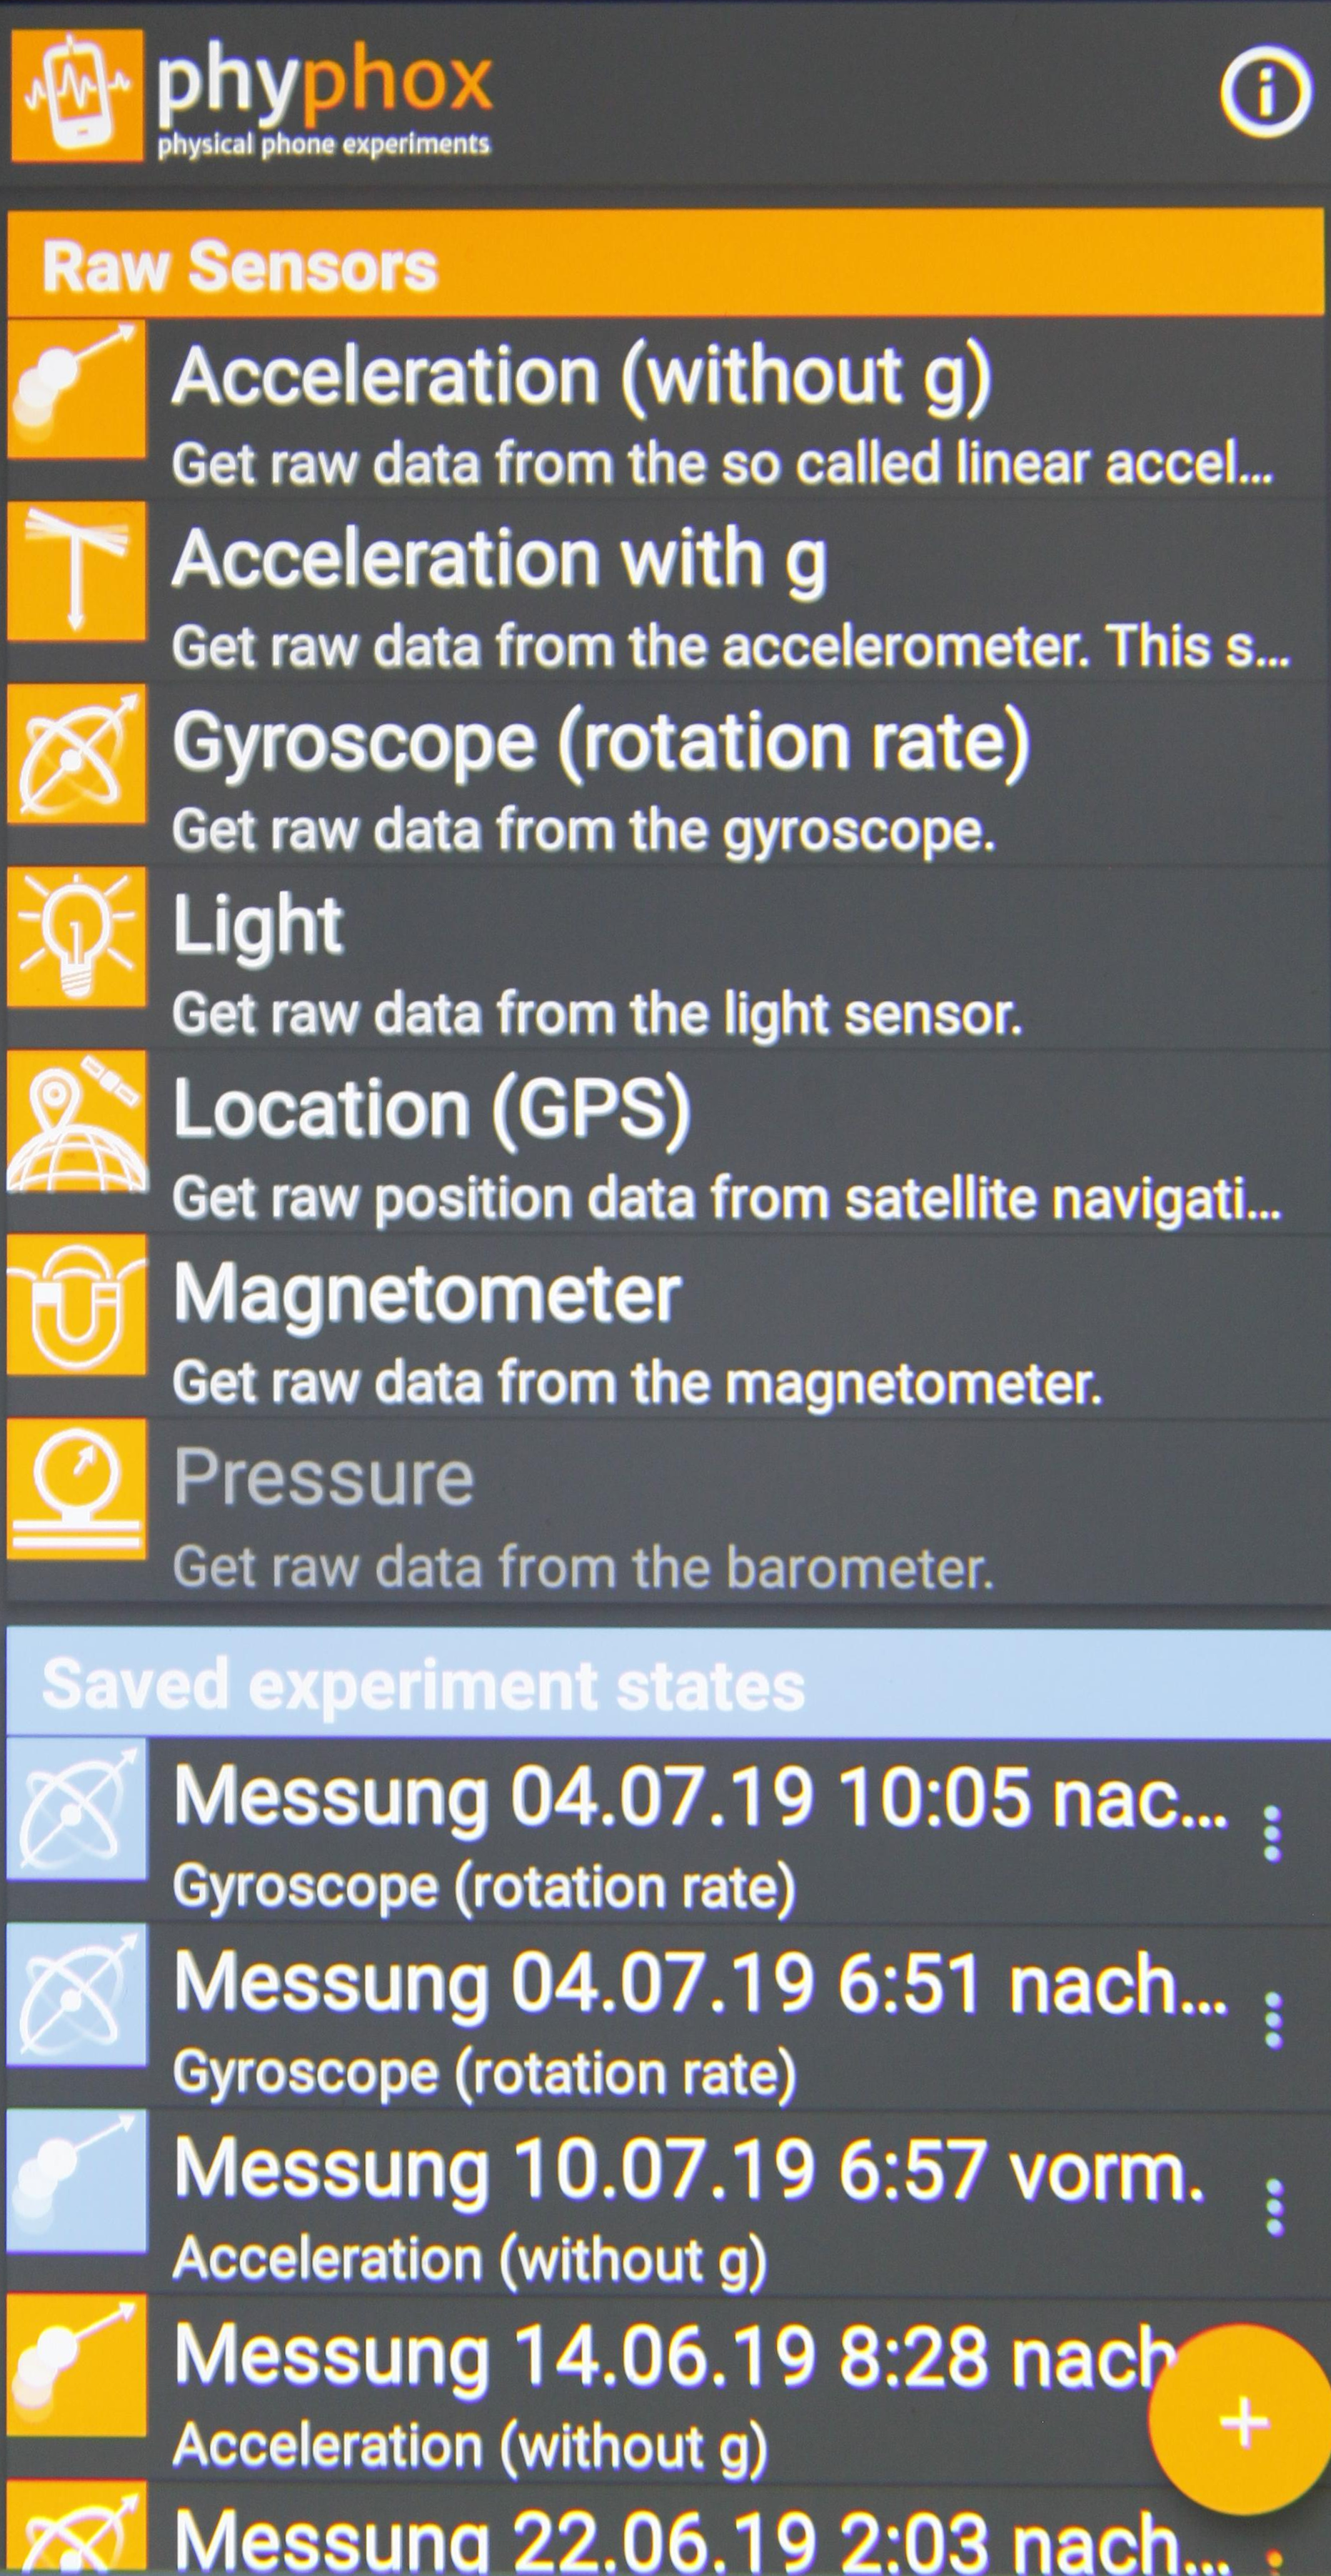
\includegraphics[width=0.25\textwidth]{phyphox_menue}\qquad%
 \raisebox{0.3truecm}{\includegraphics[width=0.65\textwidth]{phyphox_coordinates}}
\end{frame}

\begin{frame}{TGV Duplex}
 \includegraphics[width=\textwidth]{tgv-duplex}
\end{frame}

\end{document}
